
\usepackage{graphicx}
\usepackage[utf8]{inputenc}
\usepackage[english]{babel}
\usepackage{algorithm} % to write algos
\usepackage{algpseudocode} % to write algos
\usepackage{amsmath}
%\usepackage{amsfonts} % it kills \checkmark
\usepackage{amssymb}
  \usepackage[makeroom]{cancel}
%\usepackage{bm} % for bold math
\usepackage[toc,page]{appendix}
\usepackage{array}
%%BIBLIO%%
\usepackage[
    %backend=biber,
    style=numeric-comp,
    sorting=none
]{biblatex}
\usepackage{caption}
\usepackage{capt-of}
\usepackage{chemist}
\usepackage[babel]{csquotes}
\usepackage{eso-pic}
\usepackage{fancyhdr} % for headers and footers
\usepackage[Sonny]{fncychap}
\usepackage{float}
\usepackage[T1]{fontenc}
\usepackage{fullwidth}
\usepackage{gensymb}
\usepackage[left=3 cm, right=2 cm, top=2 cm, bottom=2 cm]{geometry}
\usepackage{hyperref}
  \usepackage{cleveref} % for footnote ref with hyperref 
\usepackage{enumitem} % to remove the indend of itemize with [leftmargin=*]
\usepackage{eso-pic} % For crazy background to title page
\usepackage{listings}
\usepackage{makecell}
%\usepackage{mathptmx} % curly L,% it messes with a lot of things!
\usepackage{multirow} % For multirows entry in tables
\usepackage{placeins}
\usepackage{qtree} % for trees
\usepackage{rotating} % for landscape figure
\usepackage{subcaption}
\usepackage{setspace} 
  %\doublespacing % for double spacing of main text lines
  \linespread{1.25} % equivalent to 1.5 line spacing in word
  %\linespread{1.5}  
\usepackage{tabulary}
\usepackage{tasks}
\usepackage{titlesec}
\usepackage{tcolorbox}  % for box summaries
\usepackage{wrapfig, lipsum}
\usepackage{xcolor}

% Colours
\definecolor{oxfordblue}{RGB}{0,32,68}
\definecolor{elecblue}{RGB}{0,176,240}
\definecolor{greenforest}{RGB}{34,139,34}
\definecolor{darkbrown}{RGB}{63, 42, 20}
\definecolor{darkgrey}{RGB}{105,105,105}
\definecolor{darkpink}{RGB}{219,112,147}

% Biblio
\addbibresource{mybiblio.bib}

% Ref
\hypersetup{%
    citecolor={blue},
    pdfborder={0 0 0},
    colorlinks=true,
    linkcolor=blue,
    filecolor=magenta,      
    urlcolor=blue,
	anchorcolor=red,
  linktoc=all
	%linktocpage
}

% For crazy background 
\newcommand\BackgroundPic{
  \put(-0.5cm,-0.01cm){
    \parbox[b][\paperheight]{\paperwidth}{%
      \vfill
      \centering
      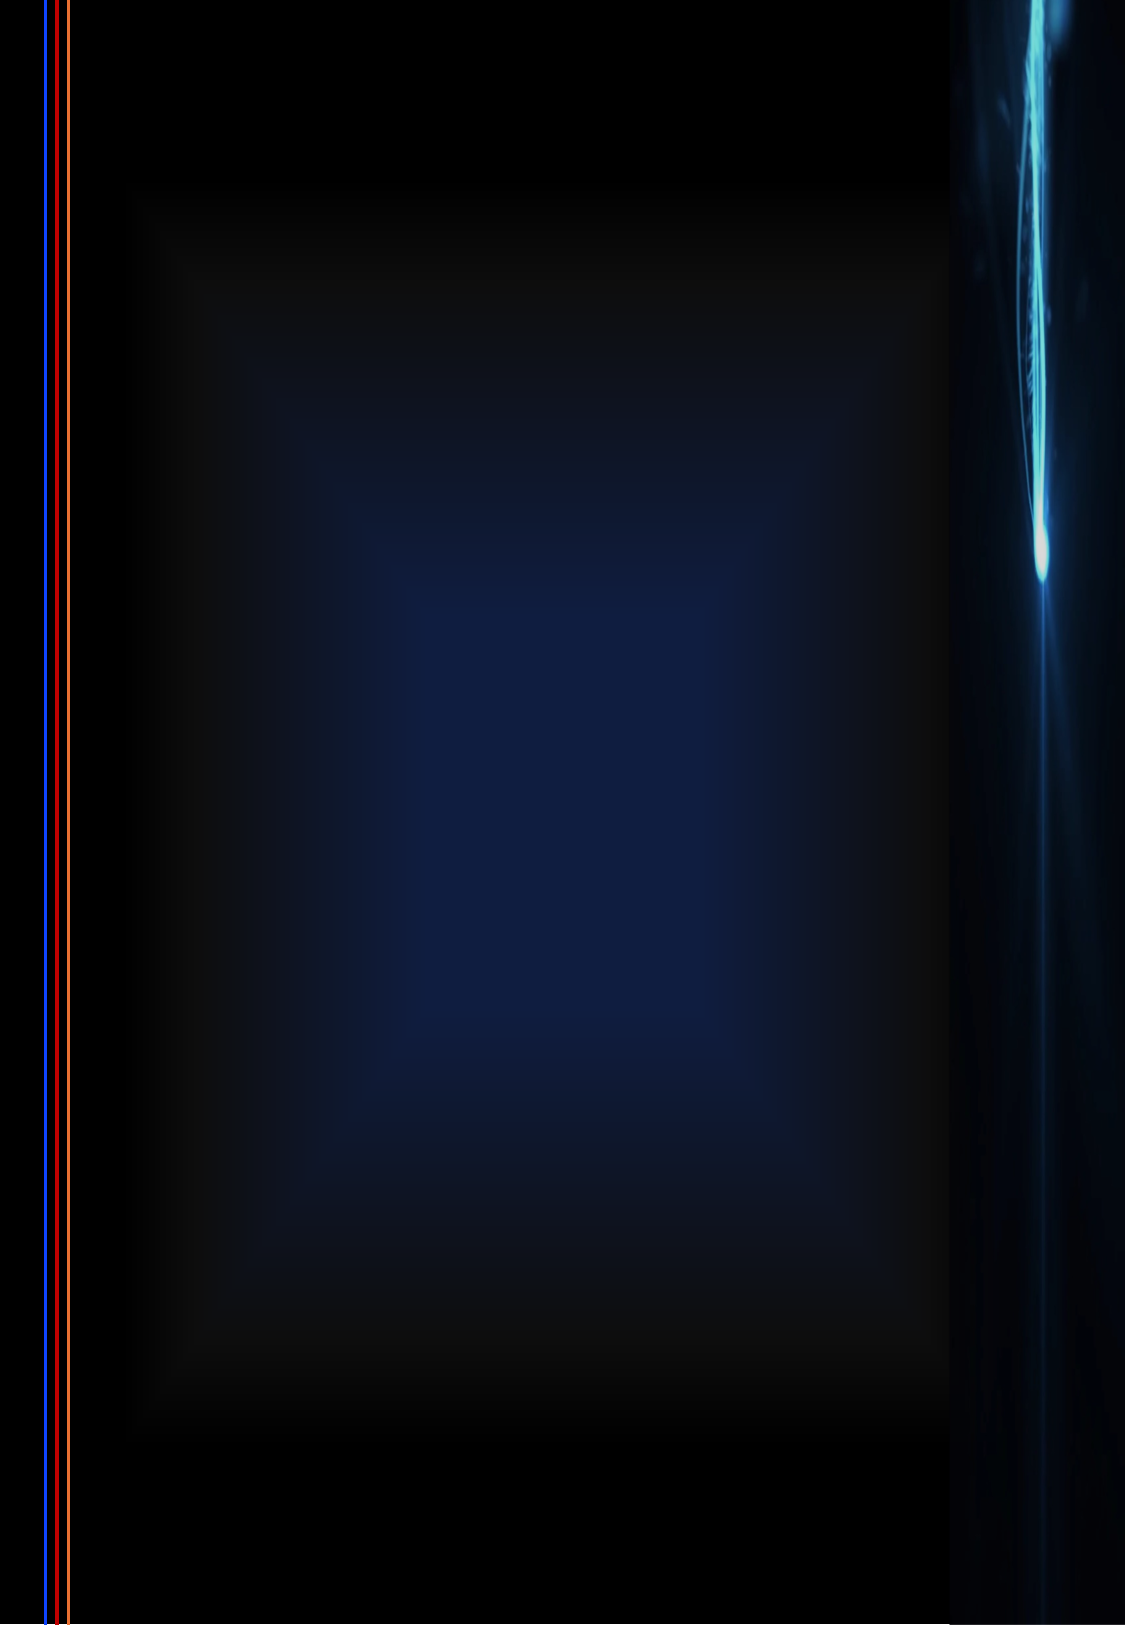
\includegraphics[width=1.05\paperwidth,height=1.02\paperheight]{Images/background3.pdf}
      \vfill
    }
  }
}

% Footnotes
\makeatletter
\newcommand\footnoteref[1]{\protected@xdef\@thefnmark{\ref{#1}}\@footnotemark}
\makeatother

\crefformat{footnote}{#2\footnotemark[#1]#3} % For the referencing of footnote


% Centred columns in table of fixed length
% Needs \usepackage{array}
\newcommand{\PreserveBackslash}[1]{\let\temp=\\#1\let\\=\temp}
\newcolumntype{C}[1]{>{\PreserveBackslash\centering}p{#1}}
\newcolumntype{R}[1]{>{\PreserveBackslash\raggedleft}p{#1}}
\newcolumntype{L}[1]{>{\PreserveBackslash\raggedright}p{#1}}
\newcolumntype{K}[1]{>{\centering\arraybackslash}p{#1}}
\newcolumntype{M}[1]{>{\centering\arraybackslash}m{#1}}
% To rotate cell in table
%\newcommand{\STAB}[1]{\begin{tabular}{@{}c@{}}#1\end{tabular}}

% For the glossary
\usepackage[acronym, nomain, nonumberlist, nopostdot, nogroupskip]{glossaries}
\usepackage{glossary-mcols}
\renewcommand*{\glspostdescription}{} % Removes dots at the end of each entry.
\renewcommand*{\glstextformat}[1]{\textcolor{black}{#1}}
%\renewcommand*{\glstextformat}[1]{\textcolor[RGB]{0,32,68}{#1}}

% Chapter style
\newcommand{\stylecolor}{\color{oxfordblue}} 
\ChNameUpperCase
\ChRuleWidth{0pt}
\ChNumVar{\stylecolor\fontsize{40}{42}\usefont{OT1}{ptm}{m}{n}\selectfont}
\ChNameVar{\stylecolor\Large\usefont{OT1}{ptm}{m}{n}\selectfont}
\ChTitleVar{\Huge\stylecolor\sc}

% Headers & Footers
\renewcommand{\chaptermark}[1]{\markboth{#1}{}}
\renewcommand{\headrulewidth}{0pt}
\fancyhf{}
\fancyhead[L]{\small \color{oxfordblue} \textbf{\textit{\textsc{Chapter \thechapter: \leftmark}}}}
\fancyhead[R]{\small \color{oxfordblue} \textbf{\textit{University of Oxford}}}
\lfoot{}
\cfoot{\thepage}
\interfootnotelinepenalty=10000
\setlength{\marginparwidth}{25mm}

\newlength\FHright
\setlength\FHright{0 mm}

\pagestyle{fancy}

% For the fancy chapter marking colour on the right
\usepackage[
  scale=1,
  angle=0,
  opacity=1,
  contents={}
]{background}
\usetikzlibrary{calc}

\pagestyle{fancy}

\newcounter{chapshift}
\addtocounter{chapshift}{-1}

% the list of colors to be used (add more if needed)
\newcommand\BoxColor{%
  %\ifcase\thechapshift blue!30\or red!30\or olive!30\or magenta!30\else yellow!30\fi}
  \ifcase\thechapshift oxfordblue\or oxfordblue\or oxfordblue\or oxfordblue\else oxfordblue\fi}

\newcommand\ChapFrame{%
  \AddEverypageHook{%
    \ifodd\value{page}
      \backgroundsetup{contents={%
        \begin{tikzpicture}[overlay,remember picture]
          \node[
            fill=\BoxColor,
            inner sep=2pt,
            rectangle,
            text width=0.8cm,
            text height=3cm,
            align=center,
            anchor=north east
          ] 
          at ($ (current page.north east) + (-0cm,-3*\thechapshift cm) $) 
          {\rotatebox{90}{\hspace*{1.35cm}\parbox[c][1.75cm][c]{3.cm}{%
              \raggedright\textcolor{white}{\scshape \vspace{0.9cm}\thechapter}}}};
        \end{tikzpicture}%
      }%
    }  
    \else
      \backgroundsetup{contents={%
        \begin{tikzpicture}[overlay,remember picture]
        \node[
          fill=\BoxColor,
          inner sep=2pt,
          rectangle,
          text width=0.8cm,
          text height=3cm,
          align=center,
          anchor=north east
        ] 
        at ($ (current page.north east) + (-0cm,-3*\thechapshift cm) $) 
        {\rotatebox{90}{\hspace*{1.35cm}\parbox[c][1.75cm][c]{3.cm}{%
            \raggedright\textcolor{white}{\scshape \vspace{0.9cm}\thechapter}}}};
        \end{tikzpicture}%
      }%
    }  
    \fi
  \BgMaterial}%
  \stepcounter{chapshift}%
}


% Useful short cut for physics:
\newcommand{\mbb}{$m_{b\bar{b}}$}
\newcommand{\mcc}{$m_{c\bar{c}}$}
\newcommand{\pt}{$p_T$}
\newcommand{\ptv}{$p_T^V$}
\newcommand{\nj}{$N_{\text{jet}}$}
\newcommand{\etm}{$E_T^{\textrm{miss}}$}


%\newcommand{\boldvhb}{$\textbf{VH(H} \rightarrow \textbf{b}\boldsymbol{\bar{b}}\textbf{)}$}
\newcommand{\boldvhb}{$\boldsymbol{VH(H \rightarrow b\bar{b})}$}
\newcommand{\boldvhc}{$\boldsymbol{VH(H \rightarrow c\bar{c})}$}
\newcommand{\boldvhbc}{$\boldsymbol{VH(H \rightarrow b\bar{b}/c\bar{c})}$}

\newcommand{\vhb}{$VH(H\rightarrow b\bar{b})$}
\newcommand{\vhc}{$VH(H\rightarrow c\bar{c})$}
\newcommand{\vhbc}{$VH(H\rightarrow b\bar{b}/c\bar{c})$}
\newcommand{\vhf}{$V+$\textit{hf}}
\newcommand{\vmf}{$V+$\textit{mf}}
\newcommand{\vlf}{$V+$\textit{lf}}
\newcommand{\whf}{$W+$\textit{hf}}
\newcommand{\wmf}{$W+$\textit{mf}}
\newcommand{\wlf}{$W+$\textit{lf}}
\newcommand{\zhf}{$Z+$\textit{hf}}
\newcommand{\zmf}{$Z+$\textit{mf}}
\newcommand{\zlf}{$Z+$\textit{lf}}
\newcommand{\ttb}{$t\bar{t}$}
\newcommand{\highdr}{High $\Delta R$}
\newcommand{\lowdr}{Low $\Delta R$}